% Cross-Modal Depth-IMU Stress Detection
% Suitable for ACM SenSys submission
% Compile with: pdflatex cross_modal_sensys.tex
%
% Required packages (add to preamble if embedding in larger paper):
%   \usepackage{tikz}
%   \usepackage{amsmath,amssymb}
%   \usepackage{booktabs}
%   \usepackage{xcolor}
%   \usetikzlibrary{arrows.meta,positioning,fit,shapes.geometric,backgrounds,calc}

\documentclass[sigconf,anonymous=false]{acmart}

\usepackage{tikz}
\usepackage{amsmath,amssymb}
\usepackage{booktabs}
\usepackage{xcolor}
\usetikzlibrary{arrows.meta,positioning,fit,shapes.geometric,backgrounds,calc}

\begin{document}

% =============================================================================
\section{Cross-Modal Stress Detection from Depth Video}
\label{sec:cross_modal}
% =============================================================================

\subsection{Problem Statement}

Continuous, passive stress monitoring in clinical environments presents a
fundamental sensing trade-off.  Inertial Measurement Unit (IMU) wristbands
offer reliable stress signatures through accelerometer-derived features---our
FLIRT-LIMU baseline achieves a test AUC of $0.89$---yet compliance is
imperfect: patients remove wearables, sensors lose contact, or deployments
simply do not include wearable instrumentation.  Depth cameras, by contrast,
are fixed infrastructure: always present, always recording, and
privacy-preserving (no RGB texture).  However, depth motion signals encode
stress far less directly than wrist acceleration, yielding a standalone
AUC of only $0.64$ under population-normalized inference.

We ask: \emph{given a cohort where both depth video and IMU data are available
during training, can we train a depth-only classifier that approaches IMU-level
performance at deployment, without requiring the IMU sensor?}

Concretely, our setting is a clinical OUD (Opioid Use Disorder) stress study
in which participants performed alternating stress and non-stress tasks while
recorded by a depth camera and a left-wrist accelerometer.
Binary stress labels follow the shared contract:
non-stress $\in \{$\texttt{jelly}, \texttt{count}, \texttt{baseline}$\}$;
stress $\in \{$\texttt{bad}, \texttt{stress}, \texttt{arithmetic},
\texttt{stroop}$\}$.
Windows of 30\,s (15\,s overlap) are extracted from each task segment,
yielding 3,040 paired (depth, IMU) windows across 62 participants.

% =============================================================================
\subsection{Approach: IMU-Guided Depth Representation Learning}
\label{sec:approach}

Our key insight is to treat the trained IMU model as a \emph{frozen teacher}
whose internal representations encode physiologically meaningful stress
patterns.  During training, the depth model is guided to produce
representations that align with those of the IMU teacher in a shared
projection space.  At deployment, the IMU branch is discarded entirely;
only the depth pathway is executed.

\subsubsection{Feature Representations}

\paragraph{Depth modality.}
Each 30\,s window yields $T=75$ depth frames (5\,Hz, 224$\times$224, top-75
entropy-selected from 150 raw frames).  Each frame is encoded by a frozen
DINOv2-ViT-B/16 encoder producing a $D=768$-dimensional embedding, giving a
window representation $\mathbf{X}_d \in \mathbb{R}^{T \times D}$.

\paragraph{IMU modality.}
Each co-registered 30\,s window of 3-axis wrist acceleration is sampled at
64\,Hz, giving a raw sequence $\mathbf{X}_i \in \mathbb{R}^{1920 \times 3}$.
FLIRT~\cite{flirt2021} hand-crafted features are computed per window, and the
absolute jelly-baseline delta is appended, yielding a 176-dimensional FLIRT
vector $\boldsymbol{\phi}(\mathbf{X}_i) \in \mathbb{R}^{176}$.  A temporal
context sequence of length $L=12$ is formed by look-back concatenation within
each (participant, task) group---replicating the input format of the trained
IMU model---producing $\mathbf{F}_i \in \mathbb{R}^{L \times 176}$.

\subsubsection{Model Architecture}

Figure~\ref{fig:pipeline} illustrates the full cross-modal training and
inference pipeline.  The architecture comprises four trainable components and
one frozen teacher.

\paragraph{Depth TCN encoder $f_\theta$.}
A Temporal Convolutional Network processes the DINOv2 frame sequence
$\mathbf{X}_d$, applying dilated causal convolutions followed by learned
attention pooling to produce a window-level depth representation:
\begin{equation}
  \mathbf{r}_d = f_\theta(\mathbf{X}_d) \in \mathbb{R}^{D_\text{TCN}}.
  \label{eq:depth_enc}
\end{equation}
The TCN encoder is \emph{warm-started} from the fold-specific checkpoint
of the standalone depth classifier, providing a strong initialisation that
already captures rudimentary stress-relevant temporal patterns.

\paragraph{Frozen IMU teacher $g_\psi$.}
A LIMU-BERT transformer~\cite{limubert2021} pre-trained via masked feature
prediction and fine-tuned for stress classification processes the FLIRT
context sequence $\mathbf{F}_i$.  The first-token representation
$\mathbf{e}_i \in \mathbb{R}^{72}$ is extracted as the teacher embedding.
All parameters $\psi$ are frozen during cross-modal training:
\begin{equation}
  \mathbf{e}_i = g_\psi(\mathbf{F}_i) \in \mathbb{R}^{72}.
  \label{eq:imu_enc}
\end{equation}

\paragraph{Per-modality input projections.}
Because depth and IMU representations have different dimensionalities
($D_\text{TCN}$ vs.\ 72), two separate linear projections map each
modality to a common shared dimension $D_s$:
\begin{equation}
  \tilde{\mathbf{r}}_d = h_d(\mathbf{r}_d), \quad
  \tilde{\mathbf{e}}_i = h_i(\mathbf{e}_i),
  \quad h_d, h_i : \mathbb{R}^{\cdot} \to \mathbb{R}^{D_s}.
  \label{eq:proj}
\end{equation}

\paragraph{Shared processing MLP $\phi_\xi$.}
The projected representations from \emph{both} modalities pass through
the \emph{same} MLP (identical weights $\xi$), enforcing a common
representational geometry:
\begin{equation}
  \mathbf{z}_d = \phi_\xi(\tilde{\mathbf{r}}_d), \quad
  \mathbf{z}_i = \phi_\xi(\tilde{\mathbf{e}}_i).
  \label{eq:shared}
\end{equation}
The shared MLP comprises LayerNorm, GELU activation, Dropout, and a linear
layer.  The same weights $\xi$ receive gradients from both the depth
classification loss and the cross-modal alignment loss, incentivising a
space in which stress-discriminative structure from the IMU teacher is
mirrored by the depth encoder.

\paragraph{Stress classifier $c_\omega$ and IMU decoder $q_\rho$.}
A two-layer MLP $c_\omega$ maps the depth shared representation to class
logits.  An optional IMU decoder $q_\rho$ reconstructs the teacher
embedding from the shared depth representation.

\subsubsection{Training Objective}

The total training loss combines three terms:
\begin{equation}
  \mathcal{L} = \mathcal{L}_\text{cls}
              + \lambda_\text{align}\,\mathcal{L}_\text{align}
              + \lambda_\text{recon}\,\mathcal{L}_\text{recon},
  \label{eq:loss}
\end{equation}
where $\lambda_\text{align}$ and $\lambda_\text{recon}$ are tuned by Optuna.

\paragraph{Classification loss.}
Standard cross-entropy on stress labels using the depth path:
\begin{equation}
  \mathcal{L}_\text{cls}
    = \text{CrossEntropy}\!\left(c_\omega(\mathbf{z}_d),\, y\right).
  \label{eq:cls}
\end{equation}

\paragraph{Cross-modal alignment loss.}
Cosine dissimilarity between the depth and IMU shared representations,
pulling the depth encoder toward the IMU representation manifold:
\begin{equation}
  \mathcal{L}_\text{align}
    = 1 - \frac{\mathbf{z}_d \cdot \mathbf{z}_i}
               {\|\mathbf{z}_d\|_2\,\|\mathbf{z}_i\|_2}.
  \label{eq:align}
\end{equation}
The IMU path ($g_\psi$, $h_i$) is frozen; gradients from
$\mathcal{L}_\text{align}$ flow only through $h_d$, $f_\theta$, and the
shared weights $\xi$ of $\phi_\xi$.

\paragraph{IMU reconstruction loss.}
When the decoder is active, the depth shared representation is required to
recover the teacher embedding:
\begin{equation}
  \mathcal{L}_\text{recon}
    = \left\| q_\rho(\mathbf{z}_d) - \mathbf{e}_i \right\|_2^2.
  \label{eq:recon}
\end{equation}
This provides a pixel-level reconstruction constraint complementary to the
distributional alignment of Eq.~\eqref{eq:align}.

\paragraph{Gradient flow summary.}  During a training step, only the depth
path parameters $\{\theta, h_d, \xi, \omega, \rho\}$ are updated.
The teacher parameters $\psi$ and $h_i$ receive no gradients.
The shared weights $\xi$ receive gradients from both $\mathcal{L}_\text{cls}$
(via $c_\omega$) and $\mathcal{L}_\text{align}$ (via the cosine term),
which jointly shape the shared space to be both stress-discriminative and
modality-aligned.

\subsection{Inference}

At deployment, only the depth camera is required.  The IMU teacher,
input projections $h_i$, and alignment losses are discarded.  Given a
30\,s depth window:
\begin{equation}
  \hat{y} = \arg\max\; c_\omega\!\left(
    \phi_\xi\!\left(h_d\!\left(f_\theta(\mathbf{X}_d)\right)\right)
  \right).
  \label{eq:infer}
\end{equation}
To mitigate inter-subject distributional shift---a dominant source of
generalisation error in participant-disjoint evaluation---we apply
\emph{subject-normalised inference}: for each test participant $s$, raw
DINOv2 frame embeddings are z-scored by that participant's own empirical
mean $\boldsymbol{\mu}_s$ and standard deviation $\boldsymbol{\sigma}_s$,
computed from their test windows (no labels used):
\begin{equation}
  \tilde{\mathbf{X}}_d^{(s)}
    = \frac{\mathbf{X}_d^{(s)} - \boldsymbol{\mu}_s}{\boldsymbol{\sigma}_s}.
  \label{eq:subj_norm}
\end{equation}

% =============================================================================
\subsection{Experimental Setup}
\label{sec:eval}

\paragraph{Evaluation protocol.}
We follow the shared evaluation contract across all modalities:
participant-disjoint folds via GroupKFold($n=5$) grouped by
\texttt{base\_subject\_id}, with inner validation via
GroupShuffleSplit(test\_size=0.2, seed=$42+\text{fold}$).
Hyperparameters are tuned with Optuna (30 trials) on fold 1 only and
evaluated on all 5 folds.  The decision threshold is selected by sweeping
19 values on the validation set and applied unchanged to the test set.

\paragraph{Metrics.}
We report test-set AUC (ROC), Balanced Accuracy (BA), Sensitivity,
Specificity, and Matthews Correlation Coefficient (MCC), averaged across
folds.  AUC is our primary metric as it is threshold-free.

% =============================================================================
\subsection{Pipeline Diagram}
\label{sec:diagram}

\begin{figure*}[t]
\centering
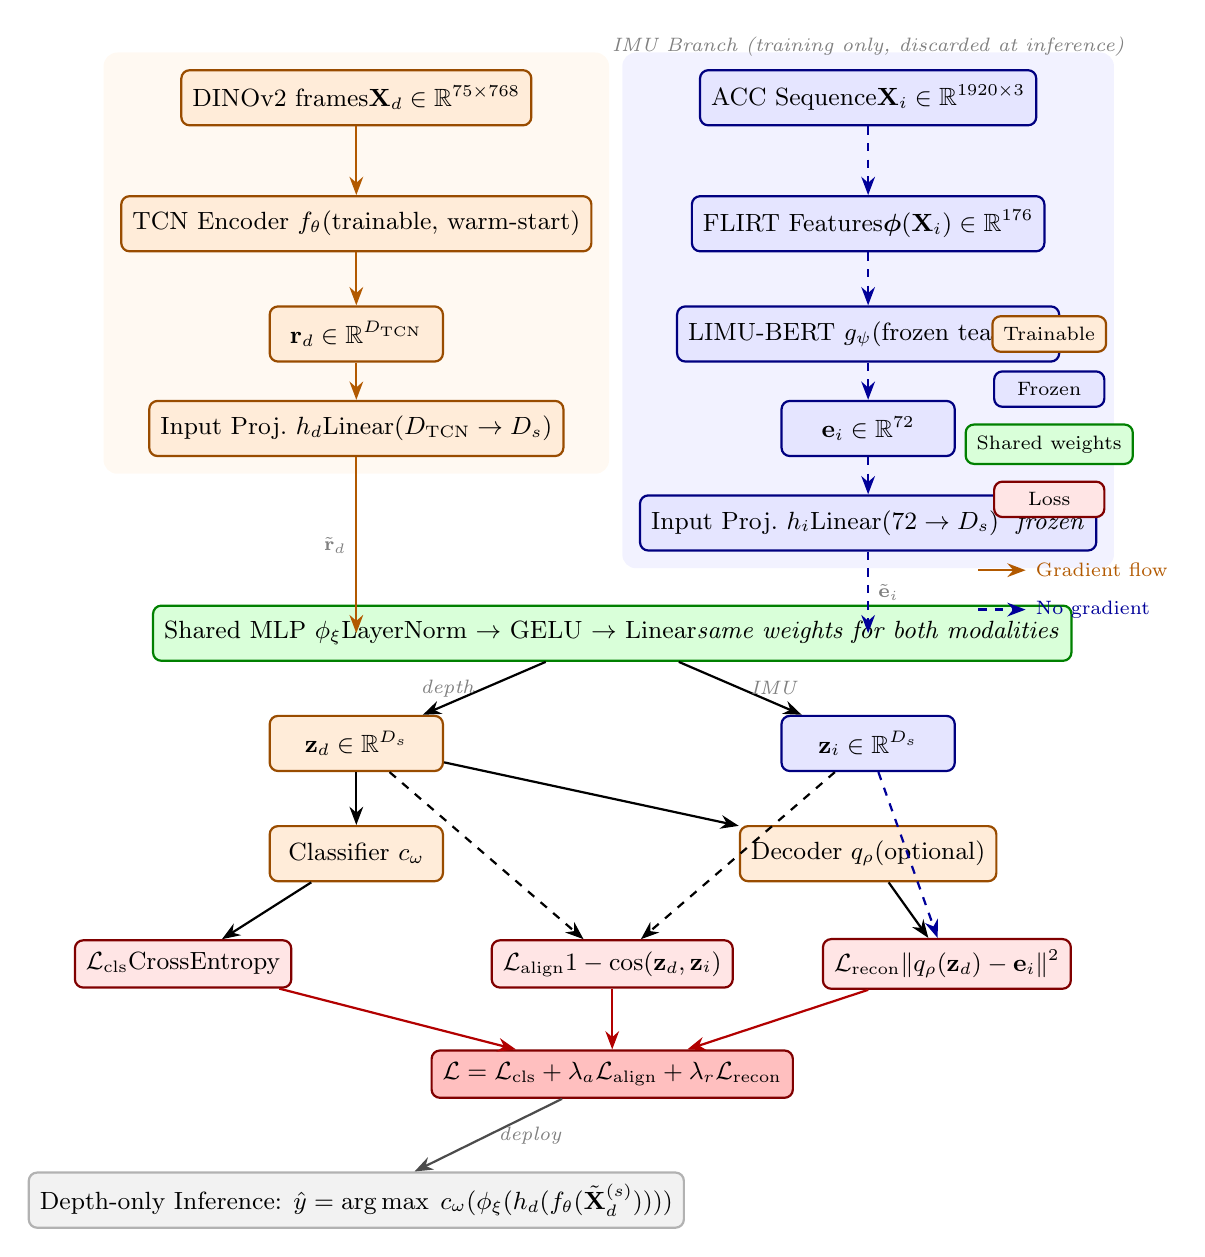
\begin{tikzpicture}[
  >=Stealth,
  font=\small,
  box/.style={
    rectangle, rounded corners=3pt, draw, thick,
    minimum width=2.2cm, minimum height=0.7cm,
    text centered, inner sep=4pt
  },
  frozen/.style={box, fill=blue!10, draw=blue!50!black},
  trainable/.style={box, fill=orange!15, draw=orange!60!black},
  shared/.style={box, fill=green!15, draw=green!50!black},
  loss/.style={box, fill=red!10, draw=red!50!black,
               minimum width=1.8cm, minimum height=0.6cm},
  arrow/.style={->, thick},
  darrow/.style={->, thick, blue!60!black, dashed},
  label/.style={font=\scriptsize\itshape, text=gray},
]

% -----------------------------------------------------------------------
% LEFT COLUMN: Depth pipeline
% -----------------------------------------------------------------------
\node[trainable] (frames)     at (0,0)      {DINOv2 frames\\$\mathbf{X}_d \in \mathbb{R}^{75\times768}$};
\node[trainable] (tcn)        at (0,-1.6)   {TCN Encoder $f_\theta$\\(trainable, warm-start)};
\node[trainable] (depth_repr) at (0,-3.0)   {$\mathbf{r}_d \in \mathbb{R}^{D_\text{TCN}}$};
\node[trainable] (hd)         at (0,-4.2)   {Input Proj.\ $h_d$\\Linear($D_\text{TCN} \to D_s$)};

% -----------------------------------------------------------------------
% RIGHT COLUMN: IMU teacher pipeline (frozen)
% -----------------------------------------------------------------------
\node[frozen] (acc)   at (6.5,0)    {ACC Sequence\\$\mathbf{X}_i \in \mathbb{R}^{1920\times3}$};
\node[frozen] (flirt) at (6.5,-1.6) {FLIRT Features\\$\boldsymbol{\phi}(\mathbf{X}_i) \in \mathbb{R}^{176}$};
\node[frozen] (limu)  at (6.5,-3.0) {LIMU-BERT $g_\psi$\\(frozen teacher)};
\node[frozen] (eimu)  at (6.5,-4.2) {$\mathbf{e}_i \in \mathbb{R}^{72}$};
\node[frozen] (hi)    at (6.5,-5.4) {Input Proj.\ $h_i$\\Linear($72 \to D_s$)\ \ \textit{frozen}};

\node[label] at (6.5, 0.65) {IMU Branch (training only, discarded at inference)};

% -----------------------------------------------------------------------
% CENTRE: Shared MLP
% -----------------------------------------------------------------------
\node[shared] (shared) at (3.25,-6.8)
  {Shared MLP $\phi_\xi$\\LayerNorm $\to$ GELU $\to$ Linear\\\textit{same weights for both modalities}};

\node[trainable] (zd) at (0,-8.2)    {$\mathbf{z}_d \in \mathbb{R}^{D_s}$};
\node[frozen]    (zi) at (6.5,-8.2)  {$\mathbf{z}_i \in \mathbb{R}^{D_s}$};

% -----------------------------------------------------------------------
% LOSSES
% -----------------------------------------------------------------------
\node[trainable] (cls_head) at (0,-9.6)    {Classifier $c_\omega$};
\node[loss]      (lcls)     at (-2.2,-11.0) {$\mathcal{L}_\text{cls}$\\CrossEntropy};
\node[loss]      (lalign)   at (3.25,-11.0) {$\mathcal{L}_\text{align}$\\$1-\cos(\mathbf{z}_d,\mathbf{z}_i)$};
\node[loss]      (lrecon)   at (7.5,-11.0)  {$\mathcal{L}_\text{recon}$\\$\|q_\rho(\mathbf{z}_d)-\mathbf{e}_i\|^2$};
\node[trainable] (decoder)  at (6.5,-9.6)   {Decoder $q_\rho$\\(optional)};

% Total loss
\node[loss, fill=red!25, minimum width=3.5cm] (ltotal) at (3.25,-12.4)
  {$\mathcal{L} = \mathcal{L}_\text{cls} + \lambda_a\mathcal{L}_\text{align} + \lambda_r\mathcal{L}_\text{recon}$};

% -----------------------------------------------------------------------
% INFERENCE PATH (bottom)
% -----------------------------------------------------------------------
\node[box, fill=gray!10, draw=gray!60] (infer) at (0,-14.0)
  {Depth-only Inference: $\hat{y} = \arg\max\; c_\omega(\phi_\xi(h_d(f_\theta(\tilde{\mathbf{X}}_d^{(s)}))))$};

% -----------------------------------------------------------------------
% ARROWS: depth branch
% -----------------------------------------------------------------------
\draw[arrow, orange!70!black] (frames)     -- (tcn);
\draw[arrow, orange!70!black] (tcn)        -- (depth_repr);
\draw[arrow, orange!70!black] (depth_repr) -- (hd);
\draw[arrow, orange!70!black] (hd)         -- (shared -| hd)
    node[midway, left, label]{$\tilde{\mathbf{r}}_d$};

% -----------------------------------------------------------------------
% ARROWS: IMU teacher branch (dashed = frozen)
% -----------------------------------------------------------------------
\draw[darrow] (acc)   -- (flirt);
\draw[darrow] (flirt) -- (limu);
\draw[darrow] (limu)  -- (eimu);
\draw[darrow] (eimu)  -- (hi);
\draw[darrow] (hi)    -- (shared -| hi)
    node[midway, right, label]{$\tilde{\mathbf{e}}_i$};

% -----------------------------------------------------------------------
% ARROWS: shared → z
% -----------------------------------------------------------------------
\draw[arrow] (shared) -- (zd)
    node[midway, left, label]{depth};
\draw[arrow] (shared) -- (zi)
    node[midway, right, label]{IMU};

% -----------------------------------------------------------------------
% ARROWS: losses
% -----------------------------------------------------------------------
\draw[arrow] (zd) -- (cls_head);
\draw[arrow] (cls_head) -- (lcls);
\draw[arrow, dashed] (zd)      -- (lalign);
\draw[arrow, dashed] (zi)      -- (lalign);
\draw[arrow] (zd)      -- (decoder);
\draw[darrow] (zi)     -- (lrecon);
\draw[arrow] (decoder) -- (lrecon);

\draw[arrow, red!70!black] (lcls)   -- (ltotal);
\draw[arrow, red!70!black] (lalign) -- (ltotal);
\draw[arrow, red!70!black] (lrecon) -- (ltotal);

% -----------------------------------------------------------------------
% ARROWS: inference
% -----------------------------------------------------------------------
\draw[arrow, gray!60!black, thick] (ltotal) -- (infer)
    node[midway, right, label]{deploy};

% -----------------------------------------------------------------------
% LEGEND
% -----------------------------------------------------------------------
\begin{scope}[shift={(8.8,-3.0)}]
  \node[trainable, minimum width=1.4cm, minimum height=0.4cm, font=\scriptsize]
    (leg1) at (0,0) {Trainable};
  \node[frozen,    minimum width=1.4cm, minimum height=0.4cm, font=\scriptsize]
    (leg2) at (0,-0.7) {Frozen};
  \node[shared,    minimum width=1.4cm, minimum height=0.4cm, font=\scriptsize]
    (leg3) at (0,-1.4) {Shared weights};
  \node[loss,      minimum width=1.4cm, minimum height=0.4cm, font=\scriptsize]
    (leg4) at (0,-2.1) {Loss};
  \node[font=\scriptsize, left=0pt of leg1] {};
  \draw[arrow, orange!70!black] (-0.9,-3.0) -- (-0.3,-3.0)
    node[right, font=\scriptsize]{Gradient flow};
  \draw[darrow]                 (-0.9,-3.5) -- (-0.3,-3.5)
    node[right, font=\scriptsize]{No gradient};
\end{scope}

% Background panels
\begin{scope}[on background layer]
  \node[fill=orange!5, rounded corners=5pt, fit=(frames)(tcn)(depth_repr)(hd),
        inner sep=6pt] {};
  \node[fill=blue!5,   rounded corners=5pt, fit=(acc)(flirt)(limu)(eimu)(hi),
        inner sep=6pt] {};
\end{scope}

\end{tikzpicture}
\caption{
  \textbf{Cross-modal depth-IMU training pipeline.}
  \textit{Training} (full diagram): depth DINOv2 frame embeddings are
  processed by a trainable TCN encoder and projected to a shared space via
  per-modality input projections.  A frozen LIMU-BERT teacher processes
  co-registered wrist accelerometer FLIRT features and maps its representation
  through the \emph{same} shared MLP weights.  Three losses shape the shared
  space: classification ($\mathcal{L}_\text{cls}$), cosine alignment
  ($\mathcal{L}_\text{align}$), and optional IMU reconstruction
  ($\mathcal{L}_\text{recon}$).
  \textit{Inference} (bottom): only the depth path is executed.
  The IMU branch is discarded entirely.
  Subject-normalised embeddings $\tilde{\mathbf{X}}_d^{(s)}$ reduce
  inter-participant distributional shift without requiring labels.
}
\label{fig:pipeline}
\end{figure*}

% =============================================================================
\subsection{Results}
\label{sec:results}

Table~\ref{tab:results} compares the cross-modal model against standalone
depth and IMU baselines under the same participant-disjoint evaluation
protocol (5-fold GroupKFold, thresholds swept on held-out validation BA).

\begin{table}[h]
\centering
\caption{Test-set performance (mean $\pm$ std across 5 participant-disjoint folds).
All cross-modal models use subject-normalised inference; the IMU branch is
discarded at test time.}
\label{tab:results}
\small
\begin{tabular}{lccc}
\toprule
\textbf{Model} & \textbf{AUC} & \textbf{BA} & \textbf{MCC} \\
\midrule
\multicolumn{4}{l}{\textit{IMU baselines (upper bound, requires wearable)}} \\
FLIRT-LSTM + Attention        & 0.890 & 0.822 & -- \\
FLIRT-LIMU-BERT               & 0.863 & 0.784 & -- \\
\midrule
\multicolumn{4}{l}{\textit{Depth-only baselines (no wearable at inference)}} \\
DINOv2-TCN, pop.\ norm        & 0.638\,$\pm$\,0.054 & 0.587\,$\pm$\,0.032 & 0.173\,$\pm$\,0.069 \\
DINOv2-TCN, subj.\ norm       & \textbf{0.717}\,$\pm$\,0.037 & 0.636\,$\pm$\,0.011 & 0.262\,$\pm$\,0.050 \\
\midrule
\multicolumn{4}{l}{\textit{Cross-modal (IMU guidance, depth-only inference)}} \\
+ cosine alignment            & 0.702\,$\pm$\,0.071 & \textbf{0.643}\,$\pm$\,0.050 & \textbf{0.249}\,$\pm$\,0.084 \\
+ GRL adversarial alignment   & 0.688\,$\pm$\,0.029 & \textbf{0.643}\,$\pm$\,0.036 & 0.250\,$\pm$\,0.053 \\
\bottomrule
\end{tabular}
\end{table}

Both cross-modal variants improve substantially over the population-normalised
depth baseline ($\text{AUC}=0.638$), reaching $0.702$ and $0.688$ respectively,
a gain of $+10.0\%$ and $+7.8\%$.
Neither variant surpasses the subject-normalised depth baseline
($\text{AUC}=0.717$), indicating that per-participant distributional
correction remains the dominant factor in this dataset.

The two alignment objectives produce a notable trade-off.
Cosine alignment achieves higher mean AUC ($0.702$ vs $0.688$) but with
substantially higher variance ($\pm 0.071$ vs $\pm 0.029$), suggesting the
rigid vector-level constraint is sensitive to fold composition.
The GRL variant produces a more calibrated classifier---sensitivity and
specificity are $0.669$/$0.617$ vs $0.696$/$0.590$---consistent with the
adversarial objective encouraging distributional rather than point-wise
alignment.
Both achieve nearly identical balanced accuracy ($0.643$) and MCC (${\approx}0.250$).

These results suggest that embedding-space alignment alone, whether
cosine-based or adversarial, transfers stress-relevant structure from the IMU
teacher but cannot replicate the inter-subject normalisation effect.
A promising direction is knowledge distillation on the teacher's output
logits (soft stress labels), which directly supervises the stress-discriminative
subspace rather than the full embedding distribution.

\end{document}
